
%(BEGIN_QUESTION)
% Copyright 2011, Tony R. Kuphaldt, released under the Creative Commons Attribution License (v 1.0)
% This means you may do almost anything with this work of mine, so long as you give me proper credit

A {\it Programmable Logic Controller} or {\it PLC} is an industrial control computer designed to input and output many types of signals.  To handle different signal types (on/off, analog, digital networking), large-scale PLCs use different ``cards'' that plug into a common frame to provide I/O capacity to the processor:

$$\includegraphics[width=15.5cm]{i02271x01.eps}$$

Read selected portions of the Allen-Bradley PLC ``1756 ControlLogix I/O Modules'' publication (document 1756-TD002A-EN-E, May 2009), and answer the following questions:

\vskip 10pt

Locate the sample 4-20 mA device wiring diagrams for the 1756-IF6CIS ``sourcing current loop analog input module'', identifying the different types of 4-20 mA field devices supported.

\vskip 10pt

Identify the rated input current range for this analog card, and also the ``count'' values associated with the low and high signal values.

\vskip 10pt

Calculate the number of counts per milliamp of signal with this analog input card, and also the resolution (mA per count).

\vskip 10pt

Calculate the ``User counts'' value for a 8.51 mA signal value input to this analog card.

\vskip 10pt

Calculate the mA current signal value at a ``User counts'' value of +4592.


\vskip 20pt \vbox{\hrule \hbox{\strut \vrule{} {\bf Suggestions for Socratic discussion} \vrule} \hrule}

\begin{itemize}
\item{} A problem-solving technique useful for making proper connections in pictorial circuit diagrams is to first identify the directions of all DC currents entering and exiting component terminals, as well as the respective voltage polarity marks (+,$-$) for those terminals, based on your knowledge of each component acting either as an electrical {\it source} or an electrical {\it load}.  Discuss and compare how these arrows and polarity marks help make sense of the sample wiring diagrams shown in this manual.
\item{} Examine the sample diagrams shown in the Rockwell manual, showing connections between 4-20 mA transmitters and the analog input channels.  Then, identify the consequences of the shielded cable in each diagram either failing {\it open} or failing {\it shorted}.
\item{} Sketch what you think are the internal components between terminals VOUT, IN, and RTN for one of the channels on the 1756-IF6CIS sourcing analog input modules, based on the recommended connections to different kinds of 4-20 mA transmitters shown in the manual.
\end{itemize}

\underbar{file i02271}
%(END_QUESTION)





%(BEGIN_ANSWER)

\noindent
{\bf Partial answer:}

\vskip 10pt

Pages 28 and 29: this card may connect to loop-powered (2-wire) 4-20 mA devices as well as self-powered (4-wire) devices.  Three connection terminals are provided per channel: a positive voltage terminal (VOUT), an input terminal (IN), and a ground (RTN).

\vskip 10pt

3106.8 counts per mA (equivalent to 0.3 microamps per count).

%(END_ANSWER)





%(BEGIN_NOTES)

Pages 28 and 29: this card may connect to loop-powered (2-wire) 4-20 mA devices as well as self-powered (4-wire) devices.  Three connection terminals are provided per channel: a positive voltage terminal (VOUT), an input terminal (IN), and a ground (RTN).

\vskip 10pt

Page 29: 0 to 21.09376 mA ; $-32768$ to +32767 counts.  This is clearly a 16-bit ADC expressing its count value as a signed integer (2's complement notation).

\vskip 10pt

${65535 \over 21.09376}= 3106.84$ counts per mA (equivalent to 0.3 microamps per count).

\vskip 10pt

8.51 mA = ${8.51 \over 21.09376}$ = 40.343\% of 65535 count span = 26439 counts above bottom = $-6329$ counts ($-6328.766312$ calculated)

\vskip 10pt

4592 counts = ${4592 - (-32768) \over 65535}$ = 57.0077\% of 21.09376 mA span = 12.02506864 mA

%INDEX% PLC, I/O: analog resolution and scaling
%INDEX% Reading assignment: Allen-Bradley 1756 ControlLogix I/O Modules publication

%(END_NOTES)

